\part{开题报告}

\section{题目}
基于MSVL的神经网络基础建模框架的设计与实现

Design and Implementation of Fundamental Modeling Framework for Neural Networks based on MSVL


\section{论文概况}
\subsection{选题来源}
国家自然科学基金项目

\subsection{摘要}

本文对神经网络的形式化建模方法进行研究,旨在为神经网络系统进行形式化验证提供模型理论基础。随着人工智能和神经网络的不断发展以及在计算机视觉,数据处理等领域的广泛应用,如何保障神经网络系统安全可靠成为了一个迫切需要解决的问题。目前,国内外关于神经网络系统安全性的研究集中在攻防方法的开发上,较少有工作使用形式化的手段对这类系统的安全性予以验证。本文以建模仿真语言MSVL以及投影时序逻辑PTL为基础,拟对神经网络的张量运算,初始化,激活函数,损失函数,优化方法等基本操作或者构件进行形式化建模研究,开发一套神经网络的基础建模框架,为CNN,RNN等其他类型的深度学习模型的形式化建模提供理论基础,为神经网络的形式化验证提供建模基础。

\section{选题依据}

\subsection{选题意义}

在如今飞速发展的机器学习和人工智能领域中,神经网络已经占据了重要地位。借助于卷积神经网络、循环神经网络等神经网络模型以及深度学习技术,神经网络系统拥有了出色的数据运算和类别预测能力。
这类系统已成功应用于计算机视觉、自然语言处理、数据挖掘等领域,具备图像分类、语音识别、数据分析、智能推荐等丰富而方便的功能。其中不乏人们所熟知的系统,如人脸识别系统、自动驾驶汽车控制系统、阿尔法围棋等。

然而,即便神经网络系统已经展示了在处理复杂问题时所取得的成功,但是它们也有其严重的安全漏洞。对于图像系统来说,具有较小扰动的对抗性样本不能为人所察觉,但是它们可以轻而易举地愚弄了神经网络模型。这种对抗攻击对神经网络系统造成了一系列威胁,也促使了这个方向上的大量研究投入。谷歌大脑也有研究表明,任何机器学习分类器都可能被欺骗,给出不正确的预测。在自动语音识别(ASR)系统中,深度循环网络已经取得了一定的成功,但是许多人已经证明,小的对抗干扰同样可以欺骗深层神经网络。

具体来说,在2016年6月,美国特斯拉公司的一辆 Model-S 型电动轿车在自动驾驶模式下撞上了一辆大型牵挂型卡车,导致一人当场身亡。事故原因是自动驾驶系统未能识别出前方卡车的白色侧面,以致没有及时启动刹车。2017年 11月的一个晚上,德国警方闯入一间公寓,因为他们接到邻居的报警,抱怨大清早就被隔壁震耳欲聋的音乐吵醒,然而这不是一个聚会,而是亚马逊的 Echo 在主人外出时,随机播放了音乐。2018年3月18日,一辆Uber自动驾驶车辆在美国亚利桑那州与一名行人相撞并致其死亡,成为全球首例自动驾驶致行人死亡事故。

值得指出的是,神经网络系统的形式化建模与验证并不是一个简单的问题。据我们了解,目前这一方面的研究工作也有限。究其原因,神经网络系统的运行依赖于由机器学习而得到的参数,其行为尚不透明、不可解释。如何为这类系统建立形式化模型以及如何对系统的安全性质进行形式化定义都是不小的挑战。此外,神经网络系统与大数据密切相关,系统的训练样本集和内部参数往往规模庞大,这无疑增加了验证的难度。神经网络系统的形式化建模与验证是一个迫切需要研究的问题,而这一问题的基础在于为神经网络建立形式化模型。

\subsection{国内外研究现状}

近年来,随着神经网络系统大规模的开发和应用,它们的安全性受到了研究人员越来越多的关注。由此开展了众多关于神经网络系统所面临的安全威胁及相应的防御技术的研究。

Szegedy 等人首次证明了可以通过对图像添加小量的人类察觉不到的扰动误导神经网络做出误分类。他们首先尝试求解让神经网络做出误分类的最小扰动的方程。但由于问题的复杂度太高,他们转而求解简化后的问题,即寻找最小的损失函数添加项,使得神经网络做出误分类,这就将问题转化成了凸优化过程。Ian J.Goodfellow 等人利用符号函数有目的地在图像样本上施加微小的扰动,提出了一种快速产生对抗样本的方法,并以高可信度在手写识别数据集上得到了验证。Moosavi-Dezfooli 等人通过迭代计算的方法生成最小规范对抗扰动,将位于分类边界内的图像逐步推到边界外,直到出现错误分类,结果证明他们生成的扰动比 FGSM 更小,同时有相似的欺骗率等。除了在神经网络系统分类任务攻击以外,还可以对自编码器和生成模型,循环神经网络,深度强化学习,语义分割和物体检测上进行攻击,攻击效果也非常可观。而在这种对抗攻击上的防御策略也主要存在三个方向,修改训练过程或者样本;修改网络;附加网络。但都未利用到形式化的手段。

近些年来,有为数不多的利用形式化手段对神经网络的攻击与防御进行验证的工作。Huang 等人通过定义一组操纵对标准样本的邻域空间离散化,由此建立一组逻辑约束,并使用可满足模理论(SMT)求解器检验标准样本邻域空间中是否存在对抗样本。同样采用 SMT 求解技术,Scheibler 等人验证了倒立摆控制系统的特定性质,如状态的可达性。然而,其神经网络规模较小,仅包含 4 层共 16 个神经元。Katz 等人提出了一种针对仅采用修正线性单元(ReLU)激活函数的深度神经网络的验证方法。该方法通
过对线性规划的单纯形法进行扩展,使其支持 ReLU 函数,进而对这类神经网络的线性性质加以验证。此外,Ghodsi 等人提出了一种对部署在云端的神经网络
系统的验证方法。该方法对神经网络的结构做出了一些限制,如数据在有穷域内、仅采用二次激活函数等,通过一定的交互式证明协议验证系统的正确性。%【基础简化的神经网络数学模型,某种限制的神经网络数学模型】

目前为止,对于神经网络的验证都是基于神经网络的朴素的数学模型,并且仅考虑了模型中特定的方面,做了特定的简化假设,进而验证特定的性质。据本人所知,目前还没有工作采用一种形式化语言对神经网络的整体进行建模。本工作正是针对现状的这一不足旨在利用MSVL这种形式化语言,对神经网络的结构、行为(包括训练和预测)进行综合性建模。为进一步验证神经网络的性质提供基础。


%目前对于神经网络系统的攻击方法大多都是基于神经网络的数值特征进行的,而常见的主被动防御措施的防御效果又很难得到保证,而利用形式化方法对神经网络系统的攻击与防御的研究又为数不多,而神经网咯的形式化建模研究更是寥寥无几。在此背景下,利用研究所开发的一种由投影时序逻辑(PTL)所定义的形式化语言:建模、仿真和验证语言(MSVL)为神经网络系统进行建模,为验证神经网络系统性质,研究神经网络系统攻防技术提供基础。



\section{研究方案}

\subsection{研究目标}
对神经网络的形式化建模进行研究,形成基础的神经网络建模理论方法,支持对神经网络的训练、测试进行综合性建模。开发BP神经网络的建模工具,该工具可由用户自定义神经网络参数,生成神经网络的综合性形式化模型。

\subsection{研究内容}
为实现上述研究目标,本文基于形式化语言MSVL,研究神经网络各要素的建模方法,具体包括以下几点。
\begin{enumerate}[(1)]
  \item 对逻辑,算数和矩阵运算进行形式化建模。
  \item 对神经网络的几种权值初始化方式进行形式化建模。
  \item 对神经网络的几种激活函数进行形式化建模。
  \item 对神经网络的几种损失函数进行形式化建模。
  \item 对神经网络的前项传播进行形式化建模。
  \item 对神经网络的反项传播进行形式化建模。
  \item 对基于梯度的优化方法进行形式化建模。
\end{enumerate}

\subsection{拟解决关键问题}
\begin{enumerate}[(1)]
  \item 如何利用基于时序逻辑的语言MSVL对神经网络进行形式化建模。
  \item 如何建立综合性的、可扩展的神经网络形式化模型。
\end{enumerate}

\subsection{拟采取的研究方法、技术路线、实验方案及可行性研究}
\begin{enumerate}[(1)]
  \item 研究方法:\\
  $\text{\quad\quad}$实验研究,对现有的理论进行创新、完善或扩充,理论扩展其应用范围,并完成
相应的模块单元测试,实现具体的模块功能。
  \item 技术路线:\\
\begin{figure}[!h]
  \centering
  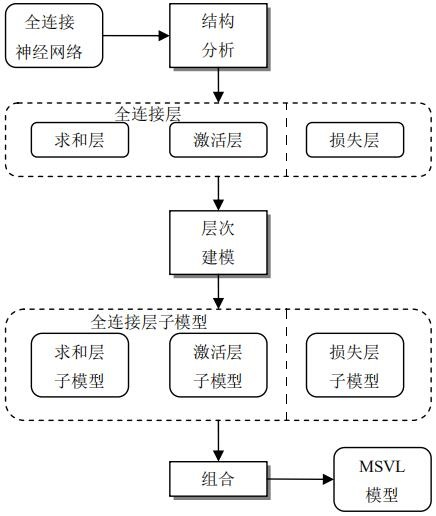
\includegraphics[width=0.5\textwidth]{FCNN.jpg}
\end{figure}

$\text{\quad\quad}$关于形式化模型的选择,拟采用基于 MSVL 语言的模型。一方面,MSVL 语言由投影时序逻辑 PTL 所定义,具备严格的逻辑基础。另一方面,该语言支持多种基本类型与复合类型,函数、框架等重要机制以及顺序、并发、选择、循环等多种控制结构,适用于此系统的建模。

$\text{\quad\quad}$神经网络系统的形式化建模从系统的结构出发,逐层开展,完整的系统模型
由各层次的模型组合而得。其核心步骤是包括数据结构和运算行为进行建模。之后的技术路线:

%\noindent \textbf{变量说明:}
%
%\begin{table}[!h]
%\resizebox{\textwidth}{!}{
%\begin{tabular}{|l|l|l|}
%\hline
%变量          & 含义           & 备注                                                                                                                           \\ \hline
%$X$           & 输入训练样本       & 维度 $N_T\times N_t$,相当于激活值矩阵$A^{(0)}$.                                                                        \\ \hline
%$X^+$           & 输入训练样本加偏置列       & 维度 $N_T\times (N_t+1)$,相当于激活值矩阵$\big(A^{(0)}\big)^+$.                                                                        \\ \hline
%$S^{(i)}$   & 第 i 层求和值矩阵 & 维度 $N_T\times N^{(i)}$, $i=1,\cdots,N,N+1$.                                                                                \\ \hline
%$A^{(i)}$   & 第 i 层激活值矩阵 & 维度 $N_T\times N^{(i)}$, $i=0,1,\cdots,N,N+1$.                                                                              \\ \hline
%$\big(A^{(i)}\big)^+$   & 第 i 层激活值矩阵加偏置列 & 维度 $N_T\times (N^{(i)}+1)$, $i=0,1,\cdots,N$.                                                                              \\ \hline
%$W^{(i)}$   & 第 i 层权值矩阵  & 维度 $N^{(i-1)}\times N^{(i)}$, $i=1,\cdots,N,N+1$.                                                                                                  \\ \hline
%$W^{(N+1)}$ & 输出层权值矩阵      & 维度 $N^{(N)}\times K$, 标签有 K 个类目。                                                                                     \\ \hline
%$W_b^{(i)}$   & 第 i 层权值偏置矩阵  & 维度 $(N^{(i-1)}+1)\times N^{(i)}$, $i=1,\cdots,N,N+1$.                                                                                                  \\ \hline
%$W_b^{(N+1)}$   &输出层权值偏置矩阵  & 维度 $(N^{(N)}+1)\times K$, 标签有 K 个类目。                                                                                                 \\ \hline
%$S^{(N+1)}$ & 输出层求和值矩阵     & 维度 $N_T\times K $.                                                                                                           \\ \hline
%$A^{(N+1)}$ & 输出层激活值矩阵     & 维度 $N_T\times K $.                                                                                                           \\ \hline
%$Y$ & 训练数据标签 & 维度 $N_T \times K$ (ONE-HOT).\\ \hline
%$\Delta^{(i)}$ & 第 i 层的反向传播中间变量矩阵 & 维度 $N_T \times N^{(i)}$, $i=1,\cdots,N,N+1$.\\ \hline
%$\Delta^{(N+1)}$ & 输出层反向传播中间变量矩阵 & 维度 $N_T \times K$.\\ \hline
%\end{tabular}}
%\end{table}


  \begin{enumerate}[(a)]
    \item 神经网络的前向传播进行建模。
 %   \begin{align*}
%   \big(A^{(0)}\big)^+W_b^{(1)}=S^{(1)}\stackrel{\sigma+b}{\longrightarrow} \big(A^{(1)}\big)^+&\Rightarrow \cdots \Rightarrow \cdots \\
%  & \Rightarrow \big(A^{(N-1)}\big)^+W_b^{(N)}=S^{(N)} \stackrel{\sigma+b}{\longrightarrow}\big(A^{(N)}\big)^+  \\
%  & \Rightarrow \big(A^{(N)}\big)^+W_b^{(N+1)}=S^{(N+1)}\stackrel{\sigma}{\longrightarrow} A^{(N+1)} \\
%  & \Rightarrow ~\mathcal{L}(A^{(N+1)},Y)
%\end{align*}
    \item 神经网络的反向传播进行建模。
%    \begin{enumerate}
%  \item 输出层权值求导:
%  \begin{align*}
%  \nabla_{W_b^{(N+1)}}\mathcal{L}(A^{(N+1)},Y) &= \frac{1}{N_T}(A^{(N)^+})^T\Delta^{(N+1)}~~~~~~\text{(矩阵化)}\\
%  \Delta^{(N+1)}& = \frac{\partial \mathcal{L}(A^{(N+1)}, Y)}{\partial A^{(N+1)}}\circ\sigma'(S^{(N+1)})\\
%  \text{当输出层使用 Soft}&\text{max+CrossEntropy 时:}\\
%  \Delta^{(N+1)} &= A^{(N+1)} - Y
%\end{align*}
%  \item 隐藏层权值求导:
%\begin{align*}
%  \nabla_{W_b^{(N)}}\mathcal{L}(A^{(N+1)},Y)&= \frac{1}{N_T}\big(A^{(N-1)^+}\big)^T\Delta^{(N)}\\
%                                \text{令:}       \Delta^{(N)} &=  \big(\Delta^{(N+1)}(W^{(N+1)})^T\big)\circ \sigma'^{(N)}(S^{(N)})\\
%    \text{\textcolor{red}{\sffamily扩展:~对于第 i 个隐藏层}}&\text{\textcolor{red}{\sffamily的权值矩阵的梯度为($i=1,2,\cdots,N.$):}}\\
%    \nabla_{W_b^{(i)}}\mathcal{L}(A^{(N+1)},Y)&= \frac{1}{N_T}\big(A^{(i-1)^+}\big)^T\Delta^{(i)}\\
%                                \text{令:}       \Delta^{(i)} &=  \Delta^{(i+1)}(W^{(i+1)})^T\circ\sigma'^{(i)}(S^{(i)})
%\end{align*}
%\end{enumerate}
    \item 对优化算法进行建模。
 %   \noindent \textbf{伪码:}\\
%$\begin{array}{l}{\text { repeat\{ }}\\ {\qquad \begin{array}{l}{\text { for } \mathrm{i}=1,11,21,31, \ldots, 991 \{}\\{~~~~~~~~\theta_{j}:=\theta_{j}-\alpha \frac{1}{10} \sum_{k=i}^{(i+9)}\left(h_{\theta}\left(x^{(k)}\right)-y^{(k)}\right) x_{j}^{(k)}} \\ { ~~~~~~\text { (for }j=0,1)} \\ ~~~~~~~~\} \\ \} \end{array}}\end{array}$
  \end{enumerate}

  \qquad例如,对于矩阵以及一个单层的神经网络课建模为如下形式化结构:
  \begin{lstlisting} [language=c]
typedef struct {
	int row, col;      // rowNum and columnNum [int]
	float** element;   // element, two dimensions
}Mat;
\end{lstlisting}
\begin{lstlisting} [language=c]
typedef struct{
	Mat ActiMat;               // active value Matrix without bias column
	Mat ActiMatPlus;           // active value Matrix with bias column
	Mat SumMat;                // sum value Matrix
	Mat WeightMat;             // weight value Matrix without bias row
	Mat WeightBiasMat;         // weight value Matrix with bias row
	Mat DeltaMat;              // backtrack temporary variable Matrix
	Mat NablaWbMat;            // gradient Matrix for weight with bias
	Mat ActiFunDerivationMat;  // active Function Dervation Matrix

	int NeuronNum;             // number of neuron [int]
	int AcitFuncNum;           // active function [int]
}FCLayer;
\end{lstlisting}
  \item 实验方案:
  \begin{enumerate}
    \item 查阅相关文献,学习投影时序逻辑的相关理论;
    \item 查阅文献和观看视频资料,学习经典神经网络的结构和建模细节;
    \item 利用MSVL进行神经网络模型搭建。
  \end{enumerate}
  \item 可行性分析:
  \begin{enumerate}
    \item 论文《MSVL a Typed Language for Temporal Logic Programming》使用逻辑定义了一种编程语言,对常用的数据类型,顺序,条件,循环结构等进行了严格的逻辑定义,并开发了一套程序语言MSVL。
    \item 论文《Full Regular Temporal Property Verification as Dynamic Pro\-gram Execution》提出了一种程序可动态执行统一模型检测方法,同 时开发了统一模型检测器 UMC4MSVL;
    \item 论文《A compiler for MSVL and its applications》基于 LLVM 完成一
个名为 MC 的编译器服务于建模仿真验证语言 MSVL,同时分析了 MC 应用
于人工智能 AI 的可行性。
  \end{enumerate}
\end{enumerate}


\subsection{研究计划及预期取得的研究成果}
\begin{table}[!h]
\resizebox{\textwidth}{!}{
\begin{tabular}{|l|l|}
\hline
时间节点            & 预期研究成果                                     \\ \hline
2020.03-2020.05   & 查阅相关文献,完成基本的调研任务,包括对 PTL 词法语法的理解;          \\ \hline
2020.05-2020.06   & 研究 MC 编译器相关的内容,了解 MSVL 相关的编程技术;            \\ \hline
2020.06-2020.08   & 研究经典深度神经网络的结构和训练细节;                        \\ \hline
2020.08-2020.10  & 完成逻辑运算,算数运算,矩阵运算的原型系统建模工作,分析并测试相关性质;       \\ \hline
2020.10-2020.12 & 完成神经网络的初始化,几种损失函数,激活函数的建模工作,分析并测试相关性质;     \\ \hline
2021.12-2021.03  & 完成神经网络的前向传播,梯度优化方式,反向传播的建模工作,并分析测试相关性质;    \\ \hline
2021.03-2021.04   & 完善整体设计的流程,改善系统框架的结构,测试并验证最终的BP神经网络工具的分类回归性能; \\ \hline
2021.04-2021.05   & 撰写论文。                                      \\ \hline
\end{tabular}}
\end{table}


\section{研究基础}
\subsection{已具备的实验条件和研究工作积累}
\begin{enumerate}
  \item 研究条件:电脑、MC 编译器、C2MSVL 转换器、UMC4MSVL 验证器。
  \item 研究工作积累:实验室具有一套完整的 PTL 模型理论,通过学习,对投影
时序逻辑有了一定的认知,并且通过查阅深度神经网络技术相关的论文,有了比较成熟的设计思路。
\end{enumerate}

\subsection{已取得的科研成果    }
无。
